\documentclass{article}
\usepackage[utf8]{inputenc}
\usepackage[russian]{babel}
\usepackage{setspace,amsmath}
\usepackage{lipsum}
\usepackage[usestackEOL]{stackengine}
\usepackage{lipsum}
\usepackage{kantlipsum}
\usepackage[left=2cm,right=2cm,top=2cm,bottom=2cm,bindingoffset=0cm]{geometry}
\usepackage[pdftex]{graphicx}
\graphicspath{{pictures/}}
\DeclareGraphicsExtensions{.pdf,.png,.jpg}
\newcommand\zz[1]{\par{\normalsize\strut #1} \hfill\ignorespaces}
\addto\captionsrussian{\def\refname{Список использованных источников}}
\begin{document}
 
\begin{center}
\textbf{
ПРАВИТЕЛЬСТВООО РОССИЙСКОЙ ФЕДЕРАЦИИ\\
НАЦИОНАЛЬНЫЙ ИССЛЕДОВАТЕЛЬСКИЙ УНИВЕРСИТЕТ\\
«ВЫСШАЯ ШКОЛА ЭКОНОМИКИ»\\
Факультет компьютерных наук
Образовательная программа «Программная инженерия»}\\
\end{center}
УДК 004.852\\
~\\
\zz{СОГЛАСНОВАНО}УТВЕРЖДАЮ
\zz{Руководитель,}Академический руководитель
\zz{доцент департамента}образовательной программы
\zz{программной инженерии}«Программная инженерия»
\zz{факультета компьютерных наук,}профессор департамента программной
\zz{канд. техн. наук}инженерии, канд. техн. наук
\zz{\noindent\rule{3cm}{0.4pt} И.В. Иванов}\noindent\rule{3cm}{0.4pt} В.В. Шилов
\zz{«\noindent\rule{1cm}{0.4pt}»\noindent\rule{2cm}{0.4pt}20\noindent\rule{0.5cm}{0.4pt}г.}«\noindent\rule{1cm}{0.4pt}»\noindent\rule{2cm}{0.4pt}20\noindent\rule{0.5cm}{0.4pt}г.
\begin{center}
\topskip=0pt
\vspace*{\fill}
\textbf{Отчет\\
по исследовательскому курсовому проекту}\\
на тему «Обучение с подкреплением для задач распределения ресурсов в облаке»\\
по направлению подготовки бакалавров 09.03.04 «Программная инженерия»\\
\vspace*{\fill}
\end{center}
{\raggedleft\vfill\Longstack[l]{%
  Выполнил:\\
  Студент группы БПИ204\\
  образовательной программы\\
  09.03.04 «Программная инженерия»\\
  Пеганов Никита Сергеевич\\
  ~\\
  \noindent\rule{6cm}{0.4pt}\\
}\par
}
\begin{center}
\vspace*{\fill}{
  Москва 2021}
\end{center}
\newpage
\begin{center}
\section {Реферат}
\end{center}
\textbf{Перечень ключевых слов: }обучение с подкреплением, reinforcement learning, RL, распределение ресурсов в облаке, облачные технологии, облачные ресурсы, Tetris, OpenAI Gym, TensorFlow, KerasRL.\\
\textbf{Краткое описание объекта исследования:} особенности выделения ресурсов при работе с облачными сервисами.\\
\textbf{Краткое описание предмета исследования:} применимость обучения с подкреплением для задачи распределения ресурсов в облаке.\\
\textbf{Цель проекта:} исследование применимости обучения с подкреплением в задачах распределения облачных ресурсов. Сравнение данного подхода с другими методами решения задачи. \\
\textbf{Метод или методология проведения работы:} метод эксперимента.\\
\textbf{Результаты проекта:}\\
\textbf{Апробация результатов:}\\
\newpage
\begin{center}
\section {Содержание}
\tableofcontents
\end{center}
\newpage
\section {Основные термины, определения и сокращения}
IT (произносится ай-ти, сокращение от англ. Information Technology) — информационные технологии\\
RL (англ. reinforcement learning) — обучение с подкреплением\\
CPU (англ. central processing unit) — электронное устройство, исполняющее машинный код программ, главная часть аппаратного обеспечения компьютера. Иногда также называется микропроцессором или процессором.
RAM (англ. Random Access Memory) — запоминающее устройство с произвольным доступом, один из видов памяти компьютера, позволяющий единовременно получить доступ к любой ячейке по её адресу на чтение или запись.
\newpage
\begin{center}
\section {Введение}
\end{center}
В первой части работы описано применение обучения с подкреплением для обучения агента самостоятельному прохождению в компьютерноц игры "Тетрис"\cite{litlink1}. Эта игра представляет собой клетчатое поле шириной 10 клеток и высотой 20 клеток. В верхней части поля друг за другом появляются клетчатые фигурки, состоящие из 4 клеток (тетрамино). Фигурки имеют форму, напоминающую форму букв "I", "Z", "L", "T", а также квадрат из четырех клеток. Пользователь имеет возможность поворачивать фигурку на 90°, а также двигать ее по горизонтали во время падения. В случае заполнения одной из строк частями фигурок строка "исчезает": все фигурки выше нее опускаются на одну строку вниз. Каждая "исчезнувшая" строка приносит игроку 1 очко.\\
Во второй части работы обучение с подкреплением применено для решения задач распределения облачных ресурсов.\\
\textbf{Актуальность}\\
Облачные технологии позволяют обеспечить круглосуточную и бесперебойную работу интернет-сервисов, что делает их востребованными во всех сферах IT-индустрии. Облачными вычислениями занимаются Amazon, Google, Huawei и другие крупнейшие информационные компании\cite{litlink2}\cite{litlink3}. В 2020 году мировой рынок облачных вычислений оценивается в 289.25 миллиардов долларов\cite{litlink4}. Распределение облачных ресурсов — одна из важнейших задач облачных вычислений.\\
\textbf{Предмет исследования}\\
Возможность использования обучения с подкреплением для решения задачи распределения ресурсов облака.
\textbf{Методы исследования}\\
Экспериментальное сравнение показателей RL в ходе решения задачи распределения облачных ресурсов с иными используемыми на практике способами. Для наглядности в работе также решена близкая задача: автоматическая игра в "Тетрис" с помощью обучения с подкреплением.  Данная компьютерная игра выбрана неслучайно: она имеет концепции, сходные с основной задачей. Во-первых, ее основная цель — упаковка фигур. В решаемой задаче так же требуется распределять задачи пользователей между имеющимися ресурсами серверов. Во-вторых, игра имеет два параметра — координаты X и Y. Основная задача так же имеет два параметра, которые требуется распределять: CPU и RAM. Также решение задачи автоматической игры в "Тетрис" позволила научиться применять использованные библиотеки и фреймворки на практике.\\
\textbf{Цели и задачи работы}\\
Определение эффективность обучения с подкреплением в задаче распределения ресурсов в облаке.\\
\textbf{Новизна и достоверность полученных результатов}\\
\textbf{Теоретическая значимость}\\
\textbf{Практическая ценность}\\
В случае превосходства RL над другими методами в рамках решения задачи распределения облачных ресурсов применение данного способа машинного обучения способно сократить нагрузку на сервера, предоставляющие доступ к облачным сервисам. Это позволит уменьшить расходы компаний на поддержку их работоспособности, а также расходы на производство при сокращении количества серверов. Проект имеет практическую ценность для экологии: уменьшение расходов электроэнергии приведет к уменьшению углеродного следа компаниий.	\\
\newpage
\begin{center}
\section {Обзор и анализ источников}
\end{center}
Первая часть курсовой работы посвящена автоматической игре в "Тетрис" с помощью обучения с подкреплением. Рассмотрим исследования данной задачи и ее решения. В статье "Tetris is Hard, Even to Approximate"\cite{litlink5} доказывается, что игра Тетрис является NP-полной задачей. Это одна из причин схожести данной игры с распределением ресурсов в облаке\cite{litlink6}. В статье Playing the Original Game Boy Tetris Using a Real Coded Genetic Algorithm\cite{litlink7} используется генетический алгоритм для симуляции игры в тетрис. В данной работе метриками успеха автор считает максимальное число удаленных строк до поражения и среднее число удаленных строк у запущенного несколько раз алгоритма. Обе метрики значительно уступают роевым оптимизациям,  продемонстрированным в работах Apply ant colony optimization to tetris\cite{litlink8} и Swarm tetris: Applying particle swarm optimization to tetris\cite{litlink9}. Примером использования RL для игры в Тетрис является статья A deep reinforcement learning bot that plays tetris\cite{litlink10}.
\newpage
\begin{center}
\section {Выбор методов, алгоритмов, моделей для решения поставленных задач}
\end{center}
Для демонстрации работы обучения с подкреплением на примере игры "Тетрис" требовалось выбрать среду для симуляции игры, а также библиотеку для реализации машинного обучения.\\
В качестве среды был рассмотрен симулятор устройства для игр "Game Boy"\ PyBoy\cite{litlink11}. Однако он был отвергнут в пользу более популярной и более простой в использовании библиотеки gym-tetris\cite{litlink12}, являющейся частью OpenAI Gym\cite{litlink13} — среды для симуляции известных компьютерных игр и физических задач.\\
При выборе библиотеки были рассмотрены pyqlearning\cite{litlink14} и Tensorforce\cite{litlink15}. Однако выбрана была библиотека KerasRL\cite{litlink16}, надстройка над фреймворком TensorFlow\cite{litlink17}. Выбор был сделан в пользу KerasRL из-за совместимости со средой OpenAI Gym.\\
В игре "Тетрис" могут быть использованы различные метрики для рассчета награды агента. Например, число убранных строк, количество сброшенных фигурок, число ходов до проигрыша, переход на новую скорость и другие. Для простоты в качестве награды было выбрано число убранных строк.
\newpage
\begin{center}
\section {Описание выбранных или предлагаемых методов, алгоритмов, моделей, методик}
\end{center}
Библиотека OpenAI Gym применяется для обучения нейронных сетей игре в различные компьютерные игры, а также решения физических задач таких, как хождение и удержание баланса. \\
TensorFlow — фреймворк с открытым кодом, совмещающий в себе передовые достижения для создания и использования нейронных сетей. Библиотека создана компанией Google, однако активно развивается сообществом программистов\cite{litlink18}.\\
Библиотека KerasRL позволяет создать нейронную сеть и агента, который будет взаимодействовать со средой и обучать сеть. Библиотека также является открытой и развивается компанией Google.\\
Для решения поставленной задачи выбран метод обучения с подкреплением. Это способ машинного обучения, при котором система, называемая агентом, обучается во время взимодействия со средой (в первой части работы средой является компьютерная игра "Тетрис"). При этом агент влияет на среду с помощью действий, а среда взаимодействует с агентом, показывая ему информацию о состоянии среды, а также возвращая награду. Цель агента — максимизация награды.\\
Заметим, что наградой в игре "Тетрис"\ может быть не только число заполненных строк. Применяются также иные метрики: количество шагов до проигрыша, средняя высота фигурок на поле во время игры и другие.\\
\begin{figure}[h]
\center{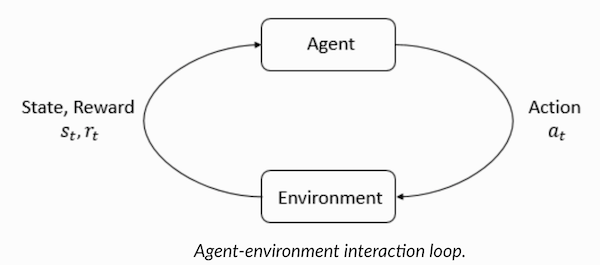
\includegraphics[width=1\linewidth]{RL_scheme}}
\caption{Схема метода обучения с подкреплением\cite{litlink19}.}
\label{ris:image}
\end{figure}
\newpage
\begin{center}
\section {Описание эксперимента}
\end{center}
В первую очередь, с помощью библиотеки OpenAI Gym создается среда, в которой обучающийся агент производит какие-либо действия. В случае, рассматриваемом в данной работе, создается среда TetrisA-v0 — эмулятор игры "Тетрис". В этой среде агент может сделать ход, передав один из вариантов действий: сдвиг фигурки влево, сдвиг фигурки вправо, поворот на 90° по часовой стрелке, против часовой стрелки, ускорение падения фигурки. При заполнении строки частями фигурок среда автоматически очищает строку и добавляет 1 к награде.\\
\begin{figure}[h]
\center{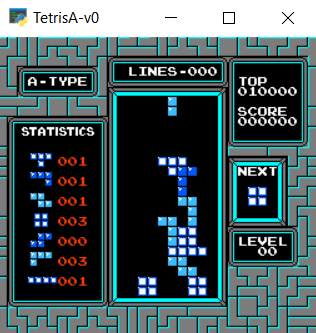
\includegraphics[width=\linewidth/2]{tetris_example}}
\caption{Пример среды TetrisA-v0.}
\label{ris:image}
\end{figure}\\
Затем с помощью библиотеки KerasRL была создана модель нейронной сети со следующими слоями. 1 слой, необходимый для сглаживания входных данных. 2 сильно связанный слой с 24 входными синапсами и функцией активации выпрямленного линейного блока. Последний сильно связанный слой имеет линейную функцию активации и 12 выходных синапсов: каждый синапс отвечает за одно из действий.\\
%ИЗМЕНИТЬ ОПИСАНИЕ СЕТИ. ДОБАВИТЬ РИСУНОК.\\
\begin{figure}[h]
\center{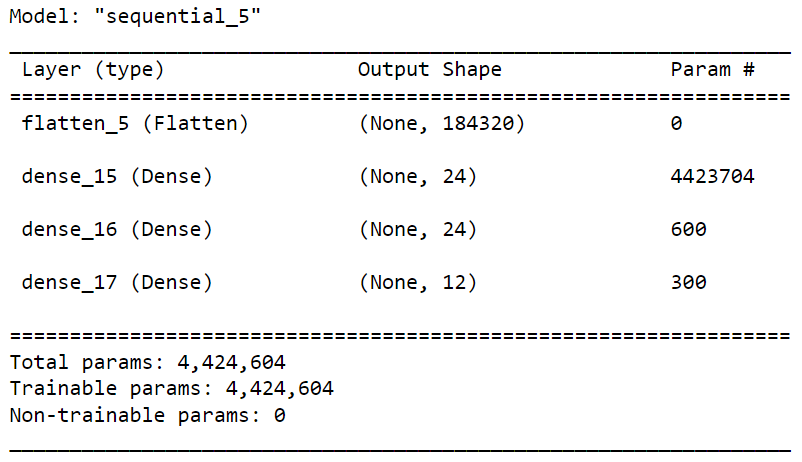
\includegraphics[width=\linewidth/2]{network}}
\caption{Краткое описание нейронной сети.}
\label{ris:image}
\end{figure}\\
На основе данной сети был создан агент с политикой BoltzmannQPolicy. Это означает, что агент вычисляет вид распределения значений, возвращаемых средой, и выбирает случайное действие на основе этого распределения.\\
После 50000 шагов, занявших 8 часов 11 минут, агент научился играть в "Тетрис" со среднем значением награды 11.02. При этом среднее число шагов до проигрыша было равно 4260.23.\\
\newpage
\begin{center}
\section {Анализ и оценка полученных результатов}
\end{center}
\newpage
\begin{center}
\section {Заключение}
\end{center}
\newpage
\begin{center}
\section {Перспективы дальнейших исследований по данной тематике}
\end{center}
\newpage
\begin{center}
\addcontentsline{toc}{section}{Список использованных источников}
\begin{thebibliography}{}
\bibitem{litlink1}  \textit{Kent, Steven} (2001) The Ultimate History of Video Games: From Pong to Pokemon: The Story Behind the Craze That Touched Our Lives and Changed the World (1st ed.). Three Rivers Press. С. 377-381. 
    \bibitem{litlink2}  \textit{Arif Mohamed} (2018) A history of cloud computing // Сайт Сomputerweekly.com. 9 апреля (https://www.computerweekly.com/feature/A-history-of-cloud-computing) Просмотрено: 11.12.2021.
    \bibitem{litlink3}  \textit{Matt Kapko} (2021) Can Huawei ‘Reinvent Itself’ as a Cloud Leader? // Сайт Sdxcentral.com. 26 апреля (https://www.sdxcentral.com/articles/news/can-huawei-reinvent-itself-as-a-cloud-leader/2021/04/) Просмотрено: 11.12.2021
    \bibitem{litlink4} \textit{Laura Wood} (2021) Global Cloud Computing Market (2020 to 2026) - by Service, Deployment, Application Type, End-user and Region Businesswire.com. 24 августа (https://www.businesswire.com/news/home/20210824005585/en/Global-Cloud-Computing-Market-2020-to-2026---by-Service-Deployment-Application-Type-End-user-and-Region---ResearchAndMarkets.com) Просмотрено: 11.12.2021
\bibitem{litlink5}  \textit{Erik D. Demaine, Susan Hohenberger, David Liben-Nowell} (2002) Tetris is Hard, Even to Approximate // Сайт Arxiv.org. 21 октября (https://arxiv.org/abs/cs/0210020) Просмотрено: 11.12.2021
\bibitem{litlink6}  \textit{Harvinder Singh, Anshu Bhasin, Parag Ravikant Kaveri} (2021) QRAS: efficient resource allocation for task scheduling in cloud computing // Сайт Researchgate.net. Апрель (https://www.researchgate.net/publication/350192028\_QRAS\_efficient\_resource\_allocation\_for\_task\_\\scheduling\_in\_cloud\_computing) Просмотрено: 11.12.2021
\bibitem{litlink7} \textit{Renan Samuel da Silva, Rafael Stubs Parpinelli} (2017) Playing the Original Game Boy Tetris Using a Real Coded Genetic Algorithm // Сайт Researchgate.net. Октрябрь (https://www.researchgate.net/publication/322321608\_Playing\_the\_Original\_Game\_Boy\_Tetris\_Using\_a\_\\Real\_Coded\_Genetic\_Algorithm) Просмотрено: 11.12.2021
\bibitem{litlink8} \textit{X. Chen, H. Wang, W. Wang, Y. Shi, and Y. Gao} (2009) Apply ant colony optimization to tetris // Сайт Dl.acm.org. 8 июля (https://dl.acm.org/doi/10.1145/1569901.1570136) Просмотрено: 11.12.2021
\bibitem{litlink9} \textit{L. Langenhoven, W. S. van Heerden, and A. P. Engelbrecht} (2010) Swarm tetris: Applying particle swarm optimization to tetris // Сайт Ieeexplore.ieee.org. 18-23 июля (https://ieeexplore.ieee.org/document/5586033) Просмотрено: 11.12.2021
\bibitem{litlink10} \textit{nuno-faria, nlinker (Nick Linker)} (2019) A bot that plays tetris using deep reinforcement learning. // Сайт Github.com. 7 сентября (https://github.com/nuno-faria/tetris-ai) Просмотрено: 11.12.2021
\bibitem{litlink11} \textit{Baekalfen (Mads Ynddal)} (2021) Game Boy emulator written in Python. // Сайт Github.com. 22 октября (https://github.com/Baekalfen/PyBoy) Просмотрено: 01.02.2022
\bibitem{litlink12} \textit{Christian Kauten} (2019) An OpenAI Gym environment for Tetris on The Nintendo Entertainment System (NES) based on the nes-py emulator. // Сайт Pypi.org. 3 июня (https://github.com/Baekalfen/PyBoy) Просмотрено: 01.02.2022
\bibitem{litlink13} \textit{OpenAI} (2021) A toolkit for developing and comparing reinforcement learning algorithms. // Сайт Github.com. 2 октября (https://github.com/openai/gym) Просмотрено: 01.02.2022
\bibitem{litlink14} \textit{accel-brain, chimera0} (2020) Reinforcement Learning Library: pyqlearning. // Сайт Pypi.org. 13 июля (https://pypi.org/project/pyqlearning/) Просмотрено: 01.02.2022
\bibitem{litlink15} \textit{Tensorforce} (2021) Tensorforce: a TensorFlow library for applied reinforcement learning. // Сайт Github.com. 30 августа (https://github.com/tensorforce/tensorforce) Просмотрено: 01.02.2022
\bibitem{litlink16} \textit{Keras-RL} (2018) Deep Reinforcement Learning for Keras. // Сайт Github.com. 1 мая (https://github.com/keras-rl/keras-rl) Просмотрено: 01.02.2022
\bibitem{litlink17} \textit{tensorflow} (2021) An Open Source Machine Learning Framework for Everyone. // Сайт Github.com. 4 ноября (https://github.com/tensorflow/tensorflow) Просмотрено: 01.02.2022
\bibitem{litlink18} \textit{Cade Metz} (2015) TensorFlow, Google's Open Source AI, Signals Big Changes in Hardware Too. // Сайт Wired.com. 10 ноября (https://www.wired.com/2015/11/googles-open-source-ai-tensorflow-signals-fast-changing-hardware-world/) Просмотрено: 02.02.2022
\bibitem{litlink19} \textit{Vihar Kurama, Samhita Alla} (2018) Обучение с подкреплением на языке Python. // Сайт Habr.com. 28 декабря (https://habr.com/ru/company/piter/blog/434738/) Просмотрено: 02.02.2022
\end{thebibliography}
\end{center}
\newpage
\begin{center}
\section {Приложения}
\end{center}
\zz{}\textbf{Приложение 1\\}
Ссылка на репозиторий проекта с исходным кодом и всеми использованными материалами.\\
https://github.com/NikPeg/Reinforcement-learning-for-resource-allocation-tasks-in-the-cloud
\end{document}